% sample.tex
\documentclass[dareport.tex]{subfiles}
\begin{document}
% Content here

\section{SAMPLE SECTION - will be removed once finalized}

Text,\footnote{Footnote text} with footnotes at bottom of page.

To conclude, the \textbf{Table 1} breakdown the program run of 4096 vertices on serial to parallel schedule \emph{dynamic} with number of processors 2, 4, 8, 16 and 32. And the \textbf{Plot 1} visualize the speedup curve of the table.
\\
\\

\begin{Large}
$S(p_{32}) =  \frac{T_{s}}{T_{p}} = \frac{49.070}{3.618} \approx 13.5627$
\end{Large}
\\
\\
$T_{s}$ = Execution time using one processor \\
$T_{p}$ = Execution time using 32 processors \\
$Load Factor$ = 4096 vertices
\\

This 2D heat transfer problem is governed by \textbf{Laplace's equation}\footnote{https://en.wikipedia.org/wiki/Laplace's\_equation} which is a second-order PDE:
\begin{center}
{\LARGE $\frac{\partial^{2}f}{\partial x^{2}} + \frac{\partial^2f}{\partial y^2} = 0$}
\end{center}


We consider the initial boundary conditions are to all zero and then the interior points of $h_{i,j}$ are where $0 < i < n, 0 < j < n$ for $(n - 1) \times (n - 1)$ interior points. The boundary points are when $i = 0, i = n, j = 0, or j = n,$ and have fixed values corresponding to the fixed temperature of the edges. And the $n$ is problem domain size. We can then compute the temperature of each interior point by iterating the equation:
\begin{center}
{\LARGE $h_{i,j} = \frac{h_{(i-1,j)} + h_{(i+1,j)} + h_{(i,j-1)} + h_{(i,j+1)}}{4}$ }
\end{center}
$(0<i<n, 0<j<n)$ for a fixed number of iterations or until the difference between iterations of a point is less than some very small precision value, e.g. Epsilon that require for the problem accuracy.
\\

Table example (see Table~\ref{eg_tbl}).

\begin{table}[h]
 \begin{center}
\begin{tabular}{|l|l|}

      \hline
      Corpus & Features\\
      \hline\hline
      AAA & 1M words\\
      BBB & spoken corpus (expensive)\\
      CCC & 2M words\\
        & free (to academics)\\
      \hline

\end{tabular}
\caption{The caption of the table}\label{eg_tbl}
 \end{center}
\end{table}


\subsection{SUBSECTION}

Text of the subsection with citations such as foster\cite{foster} quinn\cite{quinn} wendl\cite{wendl} wilkinallen\cite{wilkinallen}

\
\

For this project, I experiment with \emph{Floyd-Warshall} algorithm which is APSP and usually express in dynamic programming technique. Suppose given graph G as follow.

\begin{center}
\begin{tikzpicture}[->,>=stealth',shorten >=1pt,auto,node distance=3cm,
                    thick,main node/.style={circle,draw,font=\sffamily\Large\bfseries}]

  \node[main node] (1) {1};
  \node[main node] (2) [right of=1] {2};
  \node[main node] (3) [below of=2] {3};
  \node[main node] (4) [below of=1] {4};

  \path[every node/.style={font=\sffamily\small}]
    (1) edge node {1}  (2)
    	edge node {10} (4)
    (2) edge node {2}  (3)
    	edge node {3}  (4)
    (3) edge node {1}  (4);
\end{tikzpicture}
\end{center}

Then, the corresponding adjacency matrix is:

\begin{center}
$D_{0} = \begin{bmatrix}
        0 & 1 & \infty & 10 \\
       	\infty & 0 & 2 & 3 \\
       	\infty & \infty & 0 & 1 \\
       	\infty & \infty & \infty & 0
       	\end{bmatrix}$

\end{center}

The characteristics of \emph{Floyd-Warshall} algorithm are as follow.
\begin{itemize}
\item Finding shortest path in a weighted graph
\item Allow positive or negative edge weight
\item Do not allow negative cycle - no loop
\item Adjacency matrix as initial input - $D_{0}$
\item Contains 3-loops and has time complexity of $O(N^{3})$
\item Since adjacency matrix $D_{0}$ to given number of vertices $N$, each iteration go through intermediary vertex $k$ for the path between $i$ to $j$ vertices.
\end{itemize}
Listing \textbf{Algorithm 1} pseudocode express the steps of sequential \emph{Floyd-Warshall} algorithm for finding shortest path in a graph. In nutshell, the fundamental concept of the algorithm is to determine whether a path going from vertex $V_{i}$ to vertex $V_{j}$ via vertex $V_{k}$ is \textit{shorter than} the best-known path from vertex $V_{i}$ to vertex $V_{j}$ \cite{foster}.

\begin{center}
\begin{tikzpicture}[->,>=stealth',shorten >=1pt,auto,node distance=3cm,
                    thick,main node/.style={circle,draw,font=\sffamily\Large\bfseries}]

  \node[main node] (1) {k};
  \node[main node] (2) [below left of=1] {i};
  \node[main node] (3) [below right of=1] {j};

  \path[every node/.style={font=\sffamily\small}]
    (1) edge [bend left] node[left] {} (3)
    (2) edge [bend left] node[left] {} (1)
    	edge node {} (3);
\end{tikzpicture}
\end{center}

\textit{Illustration: The fundamental operation in Floyd-Warshall sequential shortest-path algorithm
}
\\
\\
The following is the the resultant matrix $D_{4}$ after $N$ iterations using \emph{Floyd-Warshall} algorithm.

\begin{center}
$D_{4} = \begin{bmatrix}
        0 & 1 & 3 & 4 \\
       	\infty & 0 & 2 & 3 \\
       	\infty & \infty & 0 & 1 \\
       	\infty & \infty & \infty & 0
       	\end{bmatrix}$

\end{center}

The diameter of a graph is the maximum eccentricity of any vertex in the graph\footnote{https://en.wikipedia.org/wiki/Distance\_(graph\_theory)}. In this case, the diameter of graph G is 4.
\\
\\
\\

\textbf{And example plot.}
\\
\\

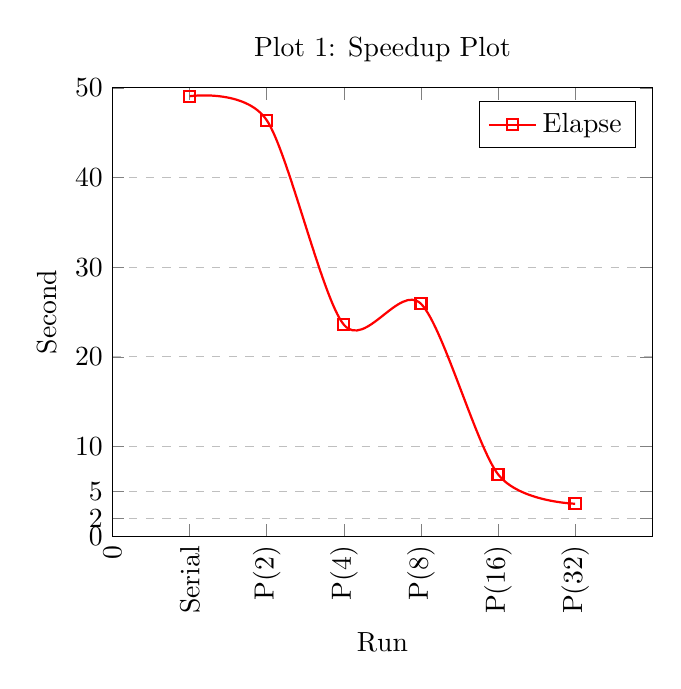
\begin{tikzpicture}
\begin{axis}[
    title={Plot 1: Speedup Plot},
    xlabel={Run},
    ylabel={Second},
    xmin=0, xmax=7,
    ymin=0, ymax=50,
    xtick={0,1,2,3,4,5,6},
    ytick={0,2,5,10,20,30,40,50},
    legend pos=north east,
    ymajorgrids=true,
    grid style=dashed,
    xticklabels={0, Serial, P(2), P(4), P(8), P(16), P(32)},
    x tick label style={rotate=90,anchor=east}
]
\addplot[
	smooth, thick, color = red,
    mark=square,
    ]
    coordinates {
    (1,49.070)(2,46.389)(3,23.588)(4,25.924)(5,6.908)(6,3.618)
    };
    \legend{Elapse}

\end{axis}
\end{tikzpicture}




\end{document}